\documentclass[a4paper, 14pt]{extarticle}
\usepackage[russian]{babel}
\usepackage[T1]{fontenc}
\usepackage{fontspec}
\usepackage{indentfirst}
\usepackage{enumitem}
\usepackage{graphicx}
\usepackage[
  left=20mm,
  right=10mm,
  top=20mm,
  bottom=20mm
]{geometry}
\usepackage{parskip}
\usepackage{titlesec}
\usepackage{xurl}
\usepackage{hyperref}
\usepackage{float}
\usepackage[
  figurename=Рисунок,
  labelsep=endash,
]{caption}
\usepackage[outputdir=build, newfloat]{minted}

\hypersetup{
  colorlinks=true,
  linkcolor=black,
  filecolor=blue,
  urlcolor=blue,
}

\renewcommand*{\labelitemi}{---}
\setmainfont{Times New Roman}
\setmonofont{JetBrains Mono}[
  SizeFeatures={Size=11},
]

\newenvironment{code}{\captionsetup{type=listing}}{}
\SetupFloatingEnvironment{listing}{name=Листинг}

\setminted{
  fontsize=\footnotesize,
  frame=lines,
  framesep=2mm,
}

\setlength{\parskip}{6pt}

\setlength{\parindent}{1cm}
\setlist[itemize]{itemsep=0em,topsep=0em,parsep=0em,partopsep=0em,leftmargin=2.0cm,wide}
\setlist[enumerate]{itemsep=0em,topsep=0em,parsep=0em,partopsep=0em,leftmargin=2.0cm,wide}

\renewcommand{\thesection}{\arabic{section}.}
\renewcommand{\thesubsection}{\thesection\arabic{subsection}.}
\renewcommand{\thesubsubsection}{\thesubsection\arabic{subsubsection}.}

\titleformat{\section}{\normalfont\bfseries}{\thesection}{0.5em}{}
\titleformat{\subsection}{\normalfont\bfseries}{\thesubsection}{0.5em}{}

\titleformat*{\section}{\normalfont\bfseries}
\titleformat*{\subsection}{\normalfont\bfseries}

\linespread{1.5}
\renewcommand{\baselinestretch}{1.5}

\begin{document}

\begin{titlepage}
  \vspace{0pt plus2fill}
  \noindent

  \vspace{0pt plus6fill}
  \begin{center}
    Санкт-Петербургский национальный исследовательский университет
    информационных технологий, механики и оптики

    \vspace{0pt plus3fill}

    Факультет инфокоммуникационных технологий

    Направление подготовки 11.03.02

    \vspace{0pt plus2fill}

    Лабораторная работа №4
  \end{center}

  \vspace{0pt plus6fill}
  \begin{flushright}
    Выполнил: \\
    Швалов Даниил Андреевич

    Группа: К33211

    Проверила: \\
    Марченко Елена Вадимовна
  \end{flushright}

  \vspace{0pt plus5fill}
  \begin{center}
    Санкт-Петербург

    2024
  \end{center}
\end{titlepage}

\section{Введение}

\textbf{Цель работы}: разработать веб-сервер, принимающий подключения по
протоколу HTTPS.

\section{Ход работы}

В качестве языка программирования, с помощью которого будет разработан
веб-сервер, был выбран язык C++, поскольку он позволяет создавать
высокопроизводительные веб-приложения, а также имеет большое количество
различных библиотек.

Для разработки сетевой части была выбрана библиотека
\foreignlanguage{english}{Boost Beast} --- одна из самых популярных библиотек
для сетевого взаимодействия по протоколу \foreignlanguage{english}{HTTP} для
C++. Для создания графического интерфейса был выбран
\foreignlanguage{english}{Qt Framework} --- кросс-платформенное и очень
популярное решение.

В ходе разработки было получено приложение, показанное на рисунке \ref{fig:1}.
При открытии приложения пользователя встречает окно, в котором ему предлагается
ввести адрес сервера, прослушиваемый порт, а также информацию, связанную с
шифрованием: файлы открытого и закрытого ключей и некоторые другие файлы. Также
есть две кнопки: запустить и остановить сервер.

\begin{figure}[H]
  \centering
  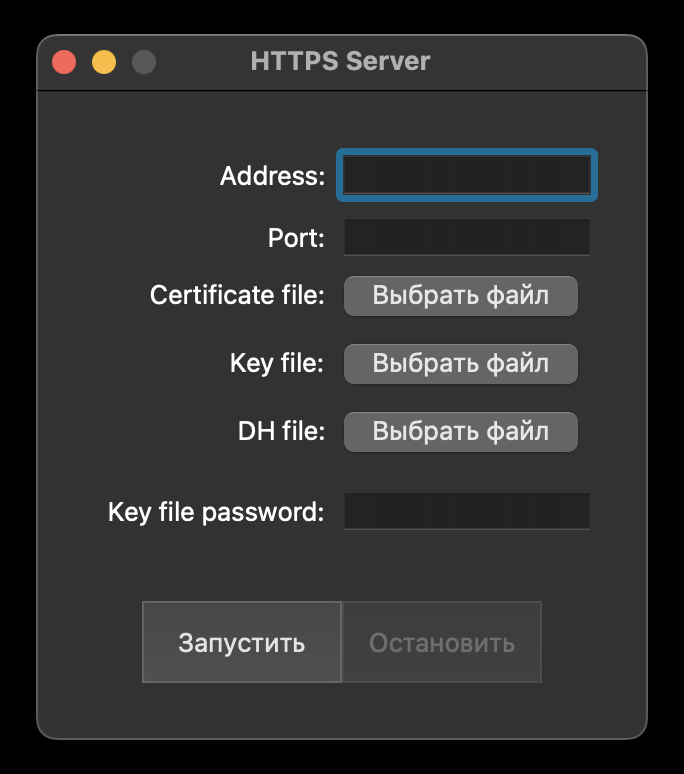
\includegraphics[width=0.33\textwidth]{images/1.png}
  \caption{Окно программы}
  \label{fig:1}
\end{figure}

В качестве серверной части был реализован эхо-сервер, т. е. сервер, который
принимает входящие соединения, считывает передаваемое содержимое и отвечает тем
же содержимым. С помощью такого простого сервера можно протестировать, работает
ли подключение по \foreignlanguage{english}{HTTPS}.

На рисунке \ref{fig:2} представлен пример настройки сервера. В качестве
прослушиваемого адреса был выбран адрес 0.0.0.0, а в качестве порта --- 8080.
Также были выбраны файлы, необходимые для шифрования. После этого была нажата
кнопка запуска сервера.

\begin{figure}[H]
  \centering
  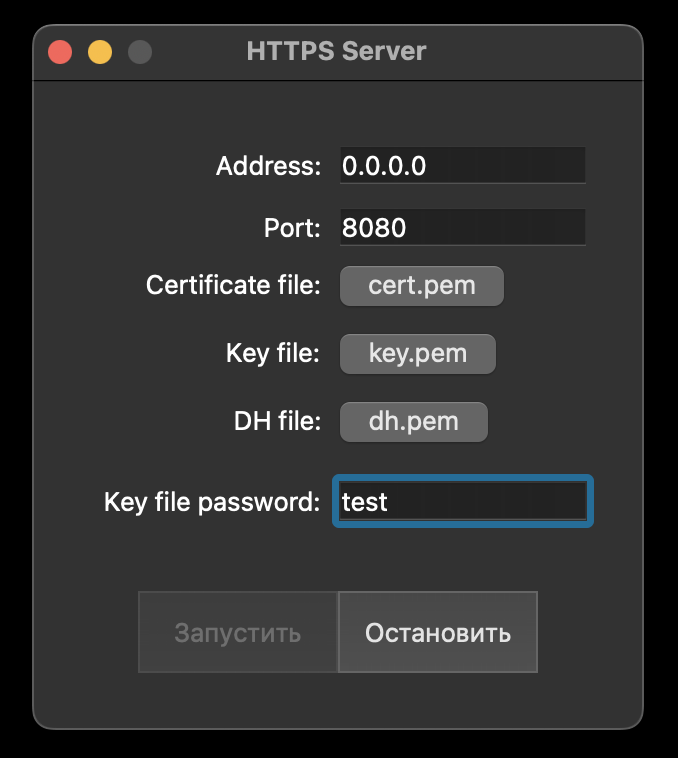
\includegraphics[width=0.33\textwidth]{images/2.png}
  \caption{Пример настройки сервера}
  \label{fig:2}
\end{figure}

Для тестирования работоспособности сервера был сделан HTTPS POST-запрос с
помощью утилиты curl. Как видно на рисунке \ref{fig:3}, подключение к серверу
прошло успешно, и сервер вернул то же самое, что и было ему отправлено.

\begin{figure}[H]
  \centering
  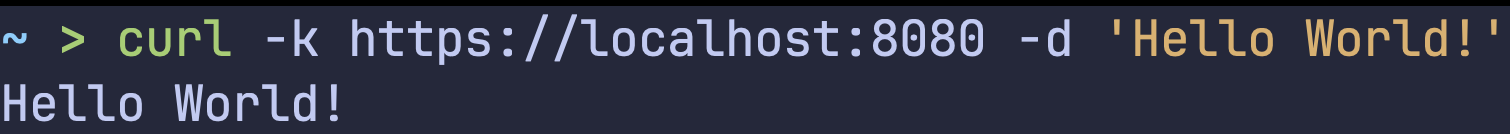
\includegraphics[width=0.9\textwidth]{images/3.png}
  \caption{Пример работы сервера}
  \label{fig:3}
\end{figure}

\section{Вывод}

В данной лабораторной работе был разработан веб-сервер, принимающий подключения
по протоколу HTTPS. Цель, поставленная в начале работы, достигнута, задачи
выполнены.

\end{document}
